\chapter{Methods}
\label{chapterlabel2}

To determine the accuracy and completeness of Burst Mode data collection it is useful to compare 3D magnetic field vectors used to steer EAS in Burst Mode (which will be called "\(B_{EAS}\)") to corresponding examples of the ground-calibrated and "true" magnetic field vectors (which will be called "\(B_{MAG}\)"). That requires data.
\\

\section{Data Access}
The online Solar Orbiter Archive (SOAR) regularly publishes science data at various processing levels from Solar Orbiter instruments including MAG and EAS where they can be accessed by the public\cite{soar}. Most science data,including MAG vector time series and EAS Burst Mode PADs, are published in CDF, which is a "Self-describing data format for the storage of scalar and multidimensional data in a platform- and discipline-independent way"\cite{cdf}. Developed by NASA Goddard Space Flight Center, CDF is close to an industry-standard data format used frequently in NASA/ESA projects\cite{horbury2020}. CDF files accommodate data fields for different variables including science data and associated metadata/support data, along with various tags and descriptions. The primary data and metadata in a CDF file can be previewed via the SOAR interface, and accessed/manipulated through freely available libraries built for Python and MATLAB\cite{cdf}.
\\

EAS and MAG data products are published to SOAR at various levels of usability; some are "raw" data directly from the instrument, and others are thoroughly processed and ready to be used in conventional, publishable research\cite{horbury2020}\cite{owen2020}\cite{zouganelis2020}. The author has previously described the data levels for EAS and MAG as follows\cite{dickson2024}:
\\

\textbf{EAS Data Levels\cite{owen2020}:}
\begin{itemize}
    \item \textbf{Level 0:} Uncalibrated CCSDS\cite{CCSDS_Standards_2022} binary data packets.
    \item \textbf{Level 1:} Uncalibrated electron count data converted to CDF in Burst Mode and Normal Mode. At this level, the MAG vectors used to steer EAS during Burst Mode (\(B_{EAS}\)) are also included.
    \item \textbf{Level 2:} Calibrated electron count data including Burst Mode PADs, but excluding \(B_{EAS}\).
    \item \textbf{Level 3:} A subset of level 2 data with additional processing.
\end{itemize}
\\

\textbf{MAG Data Levels\cite{horbury2020}:}
\begin{itemize}
    \item \textbf{Level 0:} Uncalibrated binary data.
    \item \textbf{Level 1:} Uncalibrated time series data in nT in each MAG sensor's reference frame.
    \item \textbf{Level 2:} Calibrated time series data in radial-tangent-normal (RTN), and Spacecraft Reference Frame (SRF) coordinates, corrected for offset drift and other inaccuracies, published at various cadences including E8 normal mode (8Hz) and E128 burst mode (128Hz).
    \item \textbf{Level 3:} A subset of level 2 data with additional processing.
\end{itemize}
\\

EAS level 1 Burst Mode CDF files are typically published at a rate between \(\sim\)5min/day and \(\sim\)15min/day. Some of these, published to SOAR under "solo\_L1\_swa-eas-padc\_\textit{YYYYMMdd}T\textit{hhmmss}-\textit{YYYYMMdd}T\textit{hhmmss}\_V01.cdf" are packaged with \(B_{EAS}\) as metadata in the form of normalised vectors in the SRF frame under the variable "SWA\_EAS\_MagDataUsed". 

MAG level 2 SRF CDF files, published to SOAR under "solo\_L2\_mag-srf-normal\_\textit{YYYYMMdd}\_V01", contain many hour's worth of ground-calibrated 8Hz MAG data per day (i.e. \(B_{MAG}\)), all in the same reference frame as \(B_{EAS}\) at the time of publishing (SRF), under the variable "B\_SRF".
\\

The desired CDFs were downloaded and manipulated using Python scripts with the \textit{pycdf} package in the Spacepy library. Spacepy is "a package for Python, targeted at the space sciences, that aims to make basic data analysis, modeling and visualization easier"\cite{niehof2022spacepy}. Pycdf allows individual CDF data fields to easily be referenced by name and converted to \textit{numpy} arrays as required\cite{harris2020numpy}.

\section{Time Axis Cropping}
\(B_{EAS}\) and \(B_{MAG}\) can be plotted together to yield an initial estimate of the discrepancies between them, but their respective time series are uploaded to SOAR with notably different durations (5-15 minutes vs several hours). This makes it difficult to compare one time series to the other numerically using Python, unless the longer time series is first cropped.  Several algorithms were implemented to crop magnetic field time series. Initial attempts involved simply cropping the start and end of the longer series  (\(B_{MAG}\)) to the shorter series (\(B_{EAS}\)). While this worked for some EAS CDFs (e.g. solo\_L1\_swa-eas-padc\_20231105T172733-20231105T174232\_V01.cdf and solo\_L1\_swa-eas-padc\_20230831T172734-20230831T173233\_V01.cdf), this could not be generalised to some older CDFs (e.g. solo\_L1\_swa-eas-padc\_20200624T053335-20200624T063334\_V01.cdf and solo\_L1\_swa-eas-padc\_20221201T052733-20221201T220001\_V01.cdf) whose time series began in the 1700s for the first few data points. At the time of writing, this is not signposted on SOAR, and these data points were not cropped by this algorithm. In the interest of generality, the ultimate cropping algorithm was adapted to read the timestamps in the titles of the CDFs as the start and end times to crop to, and both time series were cropped to those times instead. At present, this leads to a small amount of missing data near the start/end of a time series because the CDF filenames do not include millisecond accuracy, but this is easily fixed in the future.
\\

Once the desired start and end of an arbitrary time series are defined, an algorithm was implemented to efficiently identify the data points in that time series that should be cropped. The algorithm is summarised here:
\begin{enumerate}
    \item Determine if the time series overlaps with the desired start and stop times by performing two comparisons.
    \item If the time series overlap, then take the time in the middle of the series and determine if it is before or after the start time. 
    \item Whichever region the start time lies in, divide that region in half again and repeat N-2 times where N is the number of search divisions (typically, N=5. More divisions show diminishing returns in efficiency).
    \item Once the number of divisions has been reached, loop through the time series until the time is greater than or equal to the start time. Crop when you find the start time.
    \item Starting from the start time, loop through the time series again until the time is greater than or equal to the stop time, and then crop again.
\end{enumerate}

Implementations of this algorithm without step 6 had to loop through comparisons with every data point in a \(B_{MAG}\) time array that was several hours long. Given that the time values are saved as relatively inefficient \textit{datetime.datetime()} values, these comparisons often took \(>\)20s to complete. The inclusion of step 6 reduced this time to \(<\)2s. The core algorithm is written in Python as follows:
\\

\lstset{basicstyle=\tiny, style=myCustomMatlabStyle}
\begin{lstlisting}[language=Python]
time_index = 0
for i in range(1,searchdivisions+1):
    time_index += int(length/2**i)*(time_array[time_index+int(length/2**i)] < time_reference)
while (time_array[time_index] < time_reference) and (time_index < length-1):
    time_index += 1
\end{lstlisting}
\\

where \textit{time\_array} is the array of time values being cropped, \textit{time\_reference} is the time in \textit{time\_array} to crop at, \textit{time\_index} is an index in \textit{time\_array} within one index of \textit{time\_reference}, and \textit{length} is the length of \textit{time\_array}.
\\

As-implemented, this algorithm sometimes leads to "off by one" errors in time series length. This may be the result of comparing time series that are not using the exact same time grid, because \(B_{EAS}\) is synchronised to EAS Burst Mode time and \(B_{MAG}\) is synchronised to MAG time. In response, if \(B_{EAS}\) and \(B_{MAG}\) are not the same length after cropping, then the longer of the two time series is cropped to the shorter starting with the last data point. This may lead to some artificial time delay between the two time series.

\section{Coordinate Systems} \label{coordinate systems}

\begin{figure}[h!]
    \centering
    \centerfloat
    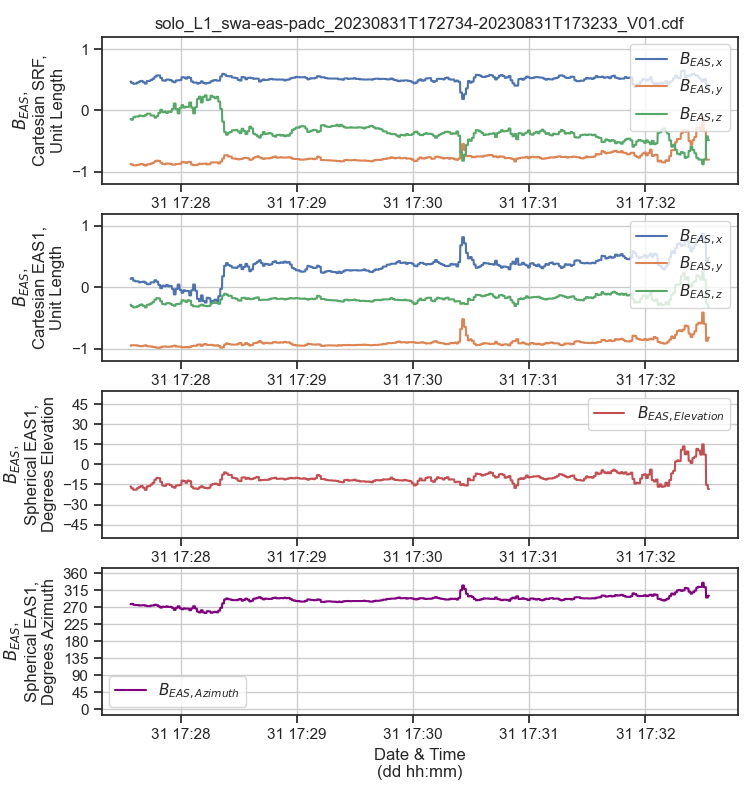
\includegraphics[width=1.05\linewidth]{figures/Transformation Example.png}
    \caption{Example \(B_{EAS}\) data from 31st August 2023. Top panel: Default cartesian \(B_{EAS}\) in SRF frame. 2nd panel: Cartesian \(B_{EAS}\) in EAS1 frame. 3rd panel: Elevation for spherical \(B_{EAS}\) in EAS1 frame. bottom panel: Azimuth for spherical \(B_{EAS}\) in EAS1 frame. The radius in spherical coordinates is not shown because all time series vectors are of length unity.}
    \caption*{Image Source: Author's own work}
    \label{fig: trans example}
\end{figure}

\(B_{EAS}\) and \(B_{MAG}\) are both acquired from SOAR in cartesian SRF coordinates. This is contrasted with data in cartesian radial-tangent-normal (RTN) coordinates (which are also provided for MAG\cite{soar}), where the "x-axis" is oriented radially away from the sun, the "z-axis" is oriented towards the north celestial pole, and the "y-axis" is tangent to a prograde orbit in the plane of the ecliptic, completing the triad. SRF coordinates are thought to correspond to the "S/C Frame" shown in figure \ref{fig: EAS schematic}, which is approximately equivalent to RTN coordinates with the "x and y" axes inverted. However, this equivalence depends on Solar Orbiter's pointing accuracy, meaning that transformations between rigidly-coupled onboard reference frames (e.g. SRF and the EAS Instrument frame in figure \ref{fig: EAS schematic}) are generally expected to be more consistent than transformations between onboard reference frames and celestial reference frames such as RTN\cite{erofeev2019}.
\\

To determine the effect of \(B_{EAS}\) and \(B_{MAG}\) on EAS elevation/azimuth binning, these time series had to be converted from cartesian SRF coordinates to spherical EAS1/EAS2 coordinates in terms of radius and elevation and azimuth angles, where the head should be chosen such that \(B_{EAS}\) and/or \(B_{MAG}\) lie within that head's FOV. This was calculated in the following order: Cartesian SRF \(\rightarrow\) Cartesian EAS1/2 \(\rightarrow\) Spherical EAS1/2. This order was chosen because SOAR provides "EAS\textit{X}\_TO\_SRF" transformation matrices packaged with level 2 EAS data CDF files published under "solo\_L2\_swa-eas\textit{X}-nm3d-dnf\_\textit{YYYYMMdd}T\textit{hhmmss}-\textit{YYYYMMdd}T\textit{hhmmss}\_V01.cdf" where \textit{X} is the EAS head number (1 or 2). Despite being packaged with timestamped CDF files, these transformation matrices do not appear to change over time (nor should they be expected to change over time). The matrices can be trivially inverted to enable a Cartesian SRF \(\rightarrow\) Cartesian EAS1/2 transformation. The default and inverted forms are shown in table \ref{tab: EASX to SRF}, as would be expected geometrically based on figure \ref{fig: EAS schematic}.
\\

\begin{table}[h!]
    \centering
    \(
    \begin{array}{cc}
        \text{EAS1 to SRF} & \text{SRF to EAS1} \\
        \begin{bmatrix}
        0 & -\frac{\sqrt{2}}{2} & +\frac{\sqrt{2}}{2}\\
        0 & +\frac{\sqrt{2}}{2} & +\frac{\sqrt{2}}{2}\\
        -1 & 0 & 0\\
        \end{bmatrix} &
        \begin{bmatrix}
        0 & 0 & -1\\
        -\frac{\sqrt{2}}{2} & +\frac{\sqrt{2}}{2} & 0\\
        +\frac{\sqrt{2}}{2} & +\frac{\sqrt{2}}{2} & 0\\
        \end{bmatrix}
        \\
        \\
        \text{EAS2 to SRF} & \text{SRF to EAS2} \\
        \begin{bmatrix}
        0 & -\frac{\sqrt{2}}{2} & +\frac{\sqrt{2}}{2}\\
        0 & -\frac{\sqrt{2}}{2} & -\frac{\sqrt{2}}{2}\\
        -1 & 0 & 0\\
        \end{bmatrix} &
        \begin{bmatrix}
        0 & 0 & -1\\
        -\frac{\sqrt{2}}{2} & -\frac{\sqrt{2}}{2} & 0\\
        +\frac{\sqrt{2}}{2} & -\frac{\sqrt{2}}{2} & 0\\
        \end{bmatrix}
        \\
        
    \end{array}
    \)\\
    \caption{A table of transformation matrices between SRF and EAS1/2 coordinates in cartesian space. The matrices in the left column were found on SOAR (in reality, \(\pm\sqrt{2}/2\) was approximated as \(\pm0.707\) on SOAR).} 
    \label{tab: EASX to SRF}
\end{table}


Once in the EAS1/2 frame, the Cartesian EAS1/2 \(\rightarrow\) Spherical EAS1/2 transformation was calculated using the \textit{astropy} library for Python; in particular, the \textit{CartesianRepresentation(x,y,z)} object with the \textit{.represent()} method\cite{astropy2013}\cite{astropy2018}\cite{astropy2022}. Figure \ref{fig: trans example} shows an example of normalised \(B_{EAS}\) data from 31st August 2023 is shown at each stage of transformation from unit cartesian SRF to unit spherical coordinates in the EAS1 frame. Since the vector time series is normalised from the start, a time series of the radius in spherical coordinates would be trivial and is omitted from figure \ref{fig: trans example}. In figure \ref{fig: trans example}, the x-axis, y-axis, and z-axis in the top panel (cartesian SRF) appear to align most closely with the z-axis (+ an offset), the y-axis (+ an offset), and the opposite of the x-axis in the 2nd panel (cartesian EAS1) respectively. This is also expected based on the "S/C" and "EAS 1 Science" frames in figure \ref{fig: EAS schematic}, further validating the matrices in table \ref{tab: EASX to SRF}.
\\


\section{Preliminary \(B_{EAS}\)-\(B_{MAG}\) Comparison}
As described in the author's earlier work, a preliminary comparison was performed between \(B_{EAS}\) and \(B_{MAG}\) from a small set of arbitrarily selected periods of Burst Mode data to justify the creation of a completeness score\cite{dickson2024}.
\\

\(B_{EAS}\) time series are stored in EAS burst mode CDF files under "SWA\_EAS\_MagDataUsed" and "EPOCH" respectively. \(B_{MAG}\) time series are stored in MAG SRF normal mode CDF files under "B\_SRF" and "EPOCH" respectively. Each "B\_SRF" vector was normalised before comparison with \(B_{EAS}\). The dot product between \(B_{EAS}\) and \(B_{MAG}\) vectors gives the angular offset between them. This angle was calculated for every vector in the sample of time series, which when plotted for 31st August 2023 yields figure \ref{fig: angle example august}.
\\

\begin{figure}[h!]
    \centering
    \centerfloat
    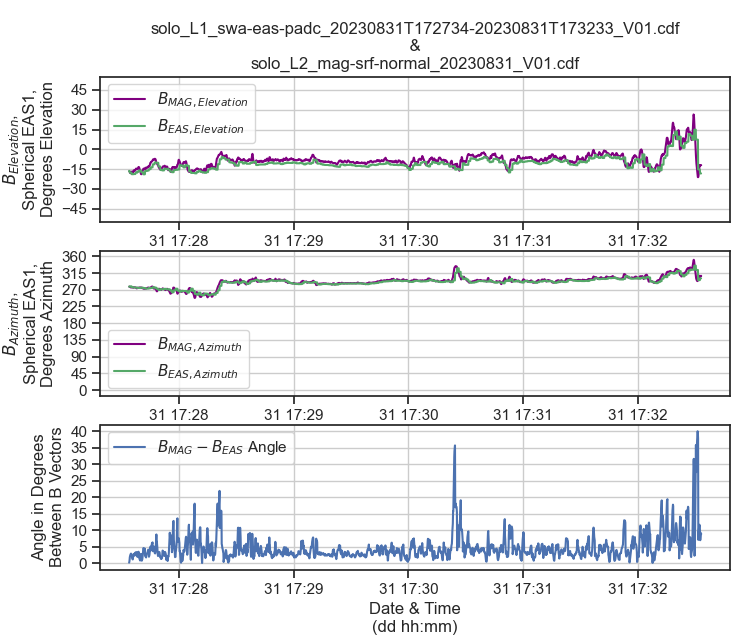
\includegraphics[width=1.05\linewidth]{figures/Angle Example.png}
    \caption{Example \(B_{EAS}\) data from a 5 minute period of EAS Burst Mode on 31st August 2023. Top panel: Elevation for \(B_{EAS}\) and \(B_{MAG}\) in spherical EAS1. Middle panel: Azimuth for \(B_{EAS}\) and \(B_{MAG}\) in spherical EAS1. Bottom panel: Angular difference between \(B_{EAS}\) and \(B_{MAG}\).}
    \caption*{Image Source: Author's own work}
    \label{fig: angle example august}
\end{figure}

\begin{figure}[h!]
    \centering
    \centerfloat
    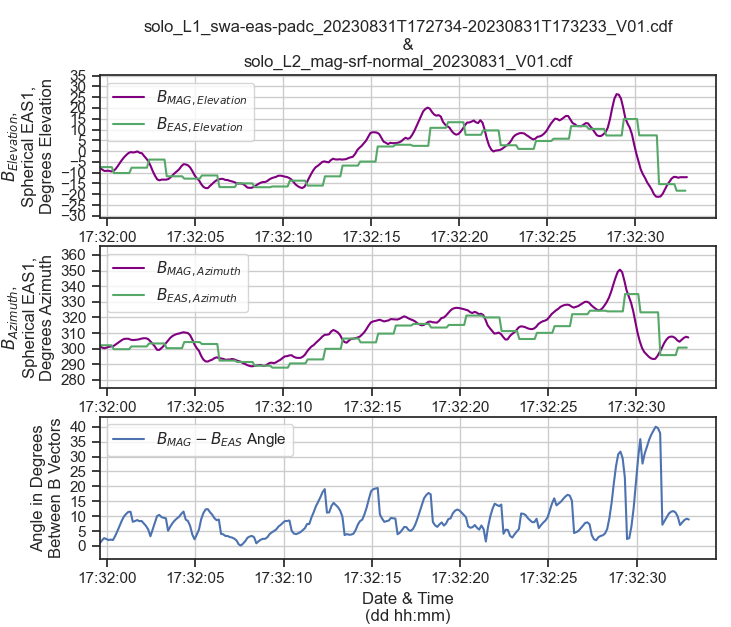
\includegraphics[width=1.05\linewidth]{figures/Angle Example Detail.png}
    \caption{A detailed look at the last \(\sim5\)s of figure \ref{fig: angle example august}. Top panel: Elevation for \(B_{EAS}\) and \(B_{MAG}\) in spherical EAS1. Middle panel: Azimuth for \(B_{EAS}\) and \(B_{MAG}\) in spherical EAS1. Bottom panel: Angular difference between \(B_{EAS}\) and \(B_{MAG}\).}
    \caption*{Image Source: Author's own work}
    \label{fig: angle example detail august}
\end{figure}

By inspection, while relatively good agreement can be seen between \(B_{EAS}\) and \(B_{MAG}\) over large timescale, there are clear discrepancies over short timescales as shown in figure \ref{fig: angle example detail august}. An unexpected observation is that \(B_{EAS}\) has less time resolution than \(B_{MAG}\), appearing only to update at 1Hz. Inspection of the raw "SWA\_EAS\_MagDataUsed" data 
By inspection, while relatively good agreement can be seen between \(B_{EAS}\) and \(B_{MAG}\) over large timescale, there are clear discrepancies over short timescales as shown in figure \ref{fig: angle example detail august}. An unexpected observation is that \(B_{EAS}\) has less time resolution than \(B_{MAG}\), appearing only to update at 1Hz. Inspection of the raw "SWA\_EAS\_MagDataUsed" time series data reveals that while this data array \textit{is} published to SOAR with 8 vectors for every second of "EPOCH" as advertised, these vectors are only updated once per second resulting in 8 identical vectors per second such that the effective cadence is 1Hz. Since these data are packaged in level 1 CDF files, they are expected to represent the true MAG data used to steer EAS, which implies that the alleged 1/8th second resolution of EAS Burst Mode is compromised by a magnetic field vector only updates at 1Hz. This will be a particular source of error during periods of fast-changing magnetic field. This effective 1Hz effect has been observed in other periods of Burst Mode from the sample including 5th November 2023 and 1st January 2023. It is absent from the relatively quiet period on 30th May 2023. Further research is required to determine the cause for this unexpectedly low update cadence.
\\

The highest angular offset in figure \ref{fig: angle example august} is observed to exceed 40\(\degree\), and it exceeds 70\(\degree\) in a different example from 5th November 2023. Otherwise, the offset is near 10\(\degree\) for most of figure \ref{fig: angle example august} and near 3\(\degree\) for a different example from 30th May 2023. Given that an individual EAS sensor head has an elevation FOV of \(\pm45\degree\) (range of 90\(\degree\)) separated into 16 bins of various sizes, the average bin width can be estimated to be \(\frac{90\degree}{16 \textrf{bins}} = 5.625\degree / \textrf{bin}\). The actual bin centers and bin widths for elevation and azimuth are tabulated with level 2 EAS data CDF files alongside the aforementioned transformation matrices. While azimuth bins are identical for both heads, elevation bins are different due to tuning of the EAS electron optics. These tables have been updated over time but remained constant since 17th July 2021. These are included in appendix \ref{appendixlabel1}. The widest angular bin in EAS1 has width \(\pm6.06\degree\). This is well below much of the angular offset observed in the sample, therefore, it is established that \(B_{EAS}\) could cause erroneous Burst Mode steering, which justifies a quality score's development.

\section{Simulating EAS Burst Mode Steering} \label{sim steering}

\begin{figure}[h!]
    \centering
    \centerfloat
    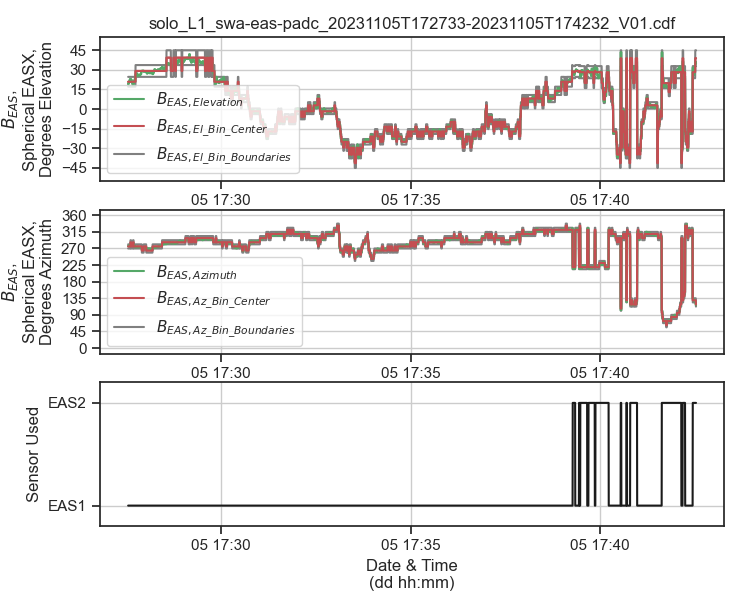
\includegraphics[width=1.05\linewidth]{figures/Steering Example.png}
    \caption{Example \(B_{EAS}\) data from a 15 minute period of EAS Burst Mode on 5th November 2023 showing a simulation of the Burst Mode steering algorithm. The reference frame for the top two panels is labeled "EASX" to indicate that it switches between EAS1 and EAS2 over the 15 minute period depending on \(B_{EAS}\) orientation and resulting head selection. Top panel: Elevation for \(B_{EAS}\) in spherical EASX, along with the centers and upper/lower bounds of the selected elevation bins ("El\_Bin\_Center" and "El\_Bin\_Boundaries" respectively). Middle panel: Azimuth for \(B_{EAS}\) in spherical EASX, along with the centers and upper/lower bounds of the selected azimuth bins ("Az\_Bin\_Center" and "Az\_Bin\_Boundaries" respectively). Bottom panel: The selected head over time.}
    \caption*{Image Source: Author's own work}
    \label{fig: steering example november}
\end{figure}

\begin{figure}[h!]
    \centering
    \centerfloat
    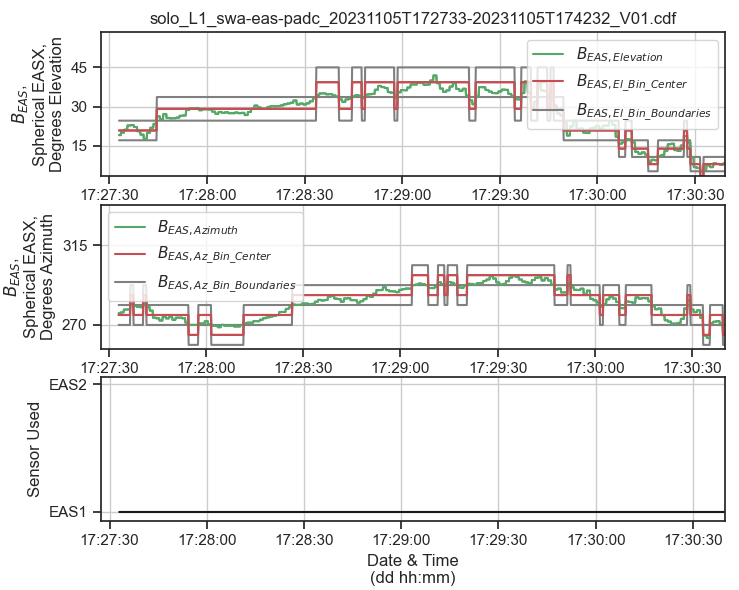
\includegraphics[width=1.05\linewidth]{figures/Steering Example Detail Start.png}
    \caption{A detailed view of the first \(\sim2.5\) minutes of figure \ref{fig: steering example november}. Top panel: Elevation + binning for \(B_{EAS}\) in spherical EASX. Middle panel: Azimuth + binning for \(B_{EAS}\) in spherical EASX. Bottom panel: The selected head over time.}
    \caption*{Image Source: Author's own work}
    \label{fig: steering example november detail}
\end{figure}

To better understand sources of error in Burst Mode data, the Burst Mode steering algorithm was simulated in Python using \(B_{EAS}\) vectors, table \ref{fig: trans example}, and the latest published binning tables shown in appendix \ref{appendixlabel1}. As per section \ref{EAS Burst Mode}, the algorithm first requires a comparison between \(B_{EAS}\) and both EAS head aperture center planes in SRF coordinates, equivalent to their z-axes + 90\degree\ elevation in their respective EAS coordinates. The smallest angle selects the EAS frame to which \(B_{EAS}\) should be transformed. Part of this algorithm is implemented in Python as follows:
\\

[insert code here]
\\

The algorithm then refers to the bin tables and selects the bins corresponding to the elevation and azimuth angles of each vector. This is implemented in Python as follows:
\\

[insert more code here]
\\

The anti-parallel vector to \(B_{EAS}\) is also determined and binned, resulting in two selected elevation bins. 
To validate the simulated binning algorithm, the time series for \(B_{EAS}\) can be plotted against the selected bin centers and upper and lower bounds. If head-selection has been performed correctly, then the \(B_{EAS}\) elevation component should never exceed \(\pm45\degree\). An example of such a plot, showing only the parallel vectors, is shown in figures \ref{fig: steering example november} and \ref{fig: steering example november detail} along with a plot of the chosen head over time, for a 15-minute period on 5th November 2023. Figure \ref{fig: steering example november} shows that the elevation and azimuth values "jump" as the reference frame switches from EAS1 to EAS2 towards the end of the time series. As expected, this switch can be triggered by the \(B_{EAS}\) elevation exceeding \(\pm45\degree\) in its previous head's reference frame. Figure \ref{fig: steering example november detail} provides a detailed view of the algorithm's selection of appropriate binning such that the \(B_{EAS}\) trace stays between bin boundaries.
\\

The most direct way to validate the algorithm is to compare the simulated bins and heads selected to the actual bins and heads selected for a given dataset. EAS level 1 Burst Mode CDF data files on SOAR provide this information. The variable "SWA\_EAS\_EasUsed" contains a time series indicating the head selected (0 for EAS1, 1 for EAS2). "SWA\_EAS\_ElevationUsed" contains a 2D time series with the bin indices (0-15) of the elevation bins selected for parallel and anti-parallel \(B_{EAS}\). "SWA\_EAS\_ELEVATION", "SWA\_EAS\_ELEVATION\_delta\_lower", and "SWA\_EAS\_ELEVATION\_delta\_upper" contain 2D time series with the actual bin centers and boundaries for the selected elevation bins (in degrees), for parallel and anti-parallel \(B_{EAS}\), and likewise for azimuth bins with "SWA\_EAS\_AZIMUTH", "SWA\_EAS\_AZIMUTH\_delta\_lower", and "SWA\_EAS\_AZIMUTH\_delta\_upper" respectively.


\section{EAS Bin Visualisation}
To facilitate the determination of Burst Mode data accuracy, a visualisation tool was developed for this project based on a plot produced by Owen et al for their 2021 publication\cite{owen2021}. This was the tool that was used to create figures \ref{fig: all bins}, \ref{fig: normal - full contours}, and \ref{fig: normal - full contours + selection} in section \ref{EAS PAD}. This visualisation is attractive because it concisely displays magnetic field vectors in SRF, circumventing the need to change coordinates following a sensor head change. The choice of SRF over RTN has been justified in section \ref{coordinate systems}. This visualisation also allows the difference in angular bin widths to be seen projected on to the sky, visualising each head and pixel's field of view along with the ensuing effects on Burst Mode steering.
\\

The visualisation was implemented in Python. The first step was to plot the grid of angular EAS bins in SRF space. Plotting the grid is easily (though inefficiently) accomplished in the EAS1/2 frame using spherical coordinates by simply plotting many closely-spaced points in straight lines along the upper and lower bounds of the elevation and azimuth bin tables (appendix \ref{appendixlabel1}). A single elevation bin can be defined by keeping the elevation angle of successive points constant (and equal to an upper/lower bound) while the azimuth phase angle is varied according to a defined angular point density, and vice versa for a single azimuth bin. Repeating this for the upper and lower edge of an elevation bin and an azimuth bin defines an elevation-azimuth pixel. Once defined, the points of each pixel can be projected to SRF space in spherical coordinates with the following sequence of transformations: Spherical EAS1/2 \(\rightarrow\) Cartesian EAS1/2 \(\rightarrow\) Cartesian SRF \(\rightarrow\) Spherical SRF. This pixel point plotting algorithm was implemented in Python as follows:
\\

\lstset{basicstyle=\tiny, style=myCustomMatlabStyle}
\begin{lstlisting}[language=Python]
angleStep = 1/pointDensity
azimuthPointCount = int(pointDensity*360/azimBinCount)
for i in range(elevBinCount):
    elevationBinWidth = 2*elevDeltaLowerArray[i]
    elevationPointCount = int(point_density*elevationBinWidth)
    binBoundaryProjectionArray.append([])
    for j in range(azimBinCount):
        pointArray = []
        for k_az in range(0,azimuthPointCount):
            lowerEdge_elev = np.array([1, elevLowerBoundArray[i], azimLowerBoundArray[j]+k_az*angleStep])
            lowerEdge_elev = cartToSphere(cart_proj_tuple[head].dot(sphereToCart(lowerEdge_elev)))
            pointArray.append(lowerEdge_elev)

            upperEdge_elev = np.array([1, elevUpperBoundArray[i], azimLowerBoundArray[j]+k_az*angleStep])
            upperEdge_elev = cartToSphere(cart_proj_tuple[head].dot(sphereToCart(upperEdge_elev)))
            pointArray.append(upperEdge_elev)

        for k_el in range(0,elevationPointCount):
            lowerEdge_azim = np.array([1, elevLowerBoundArray[i]+k_el*angleStep, azimLowerBoundArray[j]])
            lowerEdge_azim = cartToSphere(cart_proj_tuple[head].dot(sphereToCart(lowerEdge_azim)))
            pointArray.append(lowerEdge_azim)

            upperEdge_azim = np.array([1, elevLowerBoundArray[i]+k_el*angleStep, azimUpperBoundArray[j]])
            upperEdge_azim = cartToSphere(cart_proj_tuple[head].dot(sphereToCart(upperEdge_azim)))
            pointArray.append(upperEdge_azim)
\end{lstlisting}
\\

where k\_az and k\_el represent integer numbers of azimuth and elevation phase angles along a single bin edge respectively. This algorithm double-counts edges shared between adjacent pixels, trading a linear amount of computational efficiency for some convenience in plotting individual pixels. Once the points are transformed to spherical SRF coordinates, their azimuth angles are converted from the range (-180,180] to the range (0,360] for uniformity with EAS azimuth conventions. Given sufficient point density (20/\degree\ works well), this results in the mostly-continuous, visually-curved bins shown in figure \ref{fig: all bins}. Another result of high point density is that this algorithm's many matrix multiplications for each point transformation lead to a computation time of several minutes for a single image. To save time, the algorithm was adapted to save the point coordinates for each pixel to .csv files in a directory under "bin\_projections\(\backslash\)EAS\textit{X}\(\backslash\)el\textit{Y}\(\backslash\)EAS\textit{X}\_el\textit{Y}\_az\textit{Z}.csv" where \textit{X} is the EAS head number and \textit{Y} and \textit{Z} are the elevation and azimuth bin indices respectively. These files can then be read and plotted with an order of magnitude reduction in computation time. This was essentially implemented in Python as follows:
\newpage
\lstset{basicstyle=\tiny, style=myCustomMatlabStyle}
\begin{lstlisting}[language=Python]
for i in range(16):
        for j in range(32):
                filename = 'bin_projections\EAS{head}\el{i}\EAS{head}_el{i}_az{j}.csv'
                pixelArray = np.genfromtxt(filename, delimiter=",")
                el = pixelArray[1]
                az = pixelArray[2]
                ax.scatter(az,el,color=bin_color,marker='.',s=s)
\end{lstlisting}
\\

Plotting the parallel and antiparallel magnetic field vectors seen in figures \ref{fig: normal - full contours} and \ref{fig: normal - full contours + selection} was relatively simple. Since both \(B_{EAS}\) and \(B_{MAG}\) are acquired from SOAR in SRF coordinates, they only had to be transformed to spherical coordinates and plotted. To plot the contours of constant pitch angle at arbitrary pitch angles around these vectors, involved an adaptation of an algorithm written by Chris Owen in Interactive Data Language (IDL)\cite{owen2021}. The algorithm starts by constructing the cartesian transformation matrix \textit{M} from a reference frame whose z-axis is aligned with the magnetic field vector to SRF coordinates. \textit{M} is constructed as shown in table \ref{tab: Matrix M}.

\begin{table}[h!]
    \centering
    \(M=
    \begin{bmatrix}
    \cos{\phi}\cos{\theta} & \sin{\phi}\cos{\theta} & \sin{\theta}\\
    -\sin{\phi} & \cos{\phi} & 0\\
    -\cos{\phi}\sin{\theta} & -\sin{\phi}\sin{\theta} & \cos{\theta}\\
    \end{bmatrix} &
    \)\\
    \caption{The matrix \textit{M} transforming a spherical SRF vector with \(\theta=\textrm{elevation}*\pi/180\degree\) and \(\phi=\textrm{azimuth}*\pi/180\degree\) into a cartesian, field-aligned reference frame.} 
    \label{tab: Matrix M}
\end{table}
\\

From there, the the proceeding algorithm can be summarised as follows:
\begin{enumerate}
    \item 
    \item 
    \item 
\end{enumerate}

\section{Completeness Algorithm}
Research into the steering algorithm and data visualisation completed earlier in this project made it clear that there is a relatively fast approach to generating a "completeness" or "quality" score for Burst Mode PADs, circumventing the relatively expensive process of rebinning EAS Burst Mode VDF data to generate the PADs in the first place, and then assessing PAD completeness "by hand" (e.g. by counting the white bins in figure \ref{PAD example}).\\

While the binning issue described in section \ref{sim steering} affects PAD completeness, its effects are expected to be completely captured by the completeness algorithm as-is. The binning issue concerns the discrepancy between \(B_{EAS}\) and its selected bins, while the completeness algorithm concerns the discrepancy between \(B_{MAG}\) and the selected elevation bins. Whether or not these elevation bins were selected correctly only indirectly affects the completeness score depending on the agreement between \(B_{EAS}\) and \(B_{MAG}\). In fact, given sufficient disagreement between \(B_{EAS}\) and \(B_{MAG}\), the binning issue may lead \(B_{MAG}\) to be binned \textit{more accurately} than \(B_{EAS}\) (for example, if \(B_{EAS}\) is binned incorrectly while \(B_{MAG}\), by chance, is binned correctly).
\\

\blindtext

\section{S20 Link Latency}
It is possible that some of the \(B_{EAS}\)-\(B_{MAG}\) discrepancy can be attributed to latency over the S20 inter-instrument data link\cite{owen2021}.  This latency may be particularly noticeable on 1/8th second timeframe during periods of heavy data traffic\cite{owen2021}. If noticeable, then the latency is expected to cause a time delay between \(B_{EAS}\) and \(B_{MAG}\) where \(B_{MAG}\) leads by at least \(\sim\)0.125s. One approach to measuring this time delay is to perform a cross-correlation analysis between \(B_{EAS}\) and \(B_{MAG}\)\cite{hanus2019}); in principle, a cross-correlation function (CCF) takes a domain of time delays as input and the delay that gives the strongest correlation between the two time series can be selected to represent the latency. The principle behind this approach is well-illustrated by figure \ref{fig: Hanus CCF} by Hanus et al\cite{hanus2019} for two 1D time series \(x(t)\) and \(z(t)\) and latency \(\tau_0\).

\begin{figure}[h!]
    \centering
    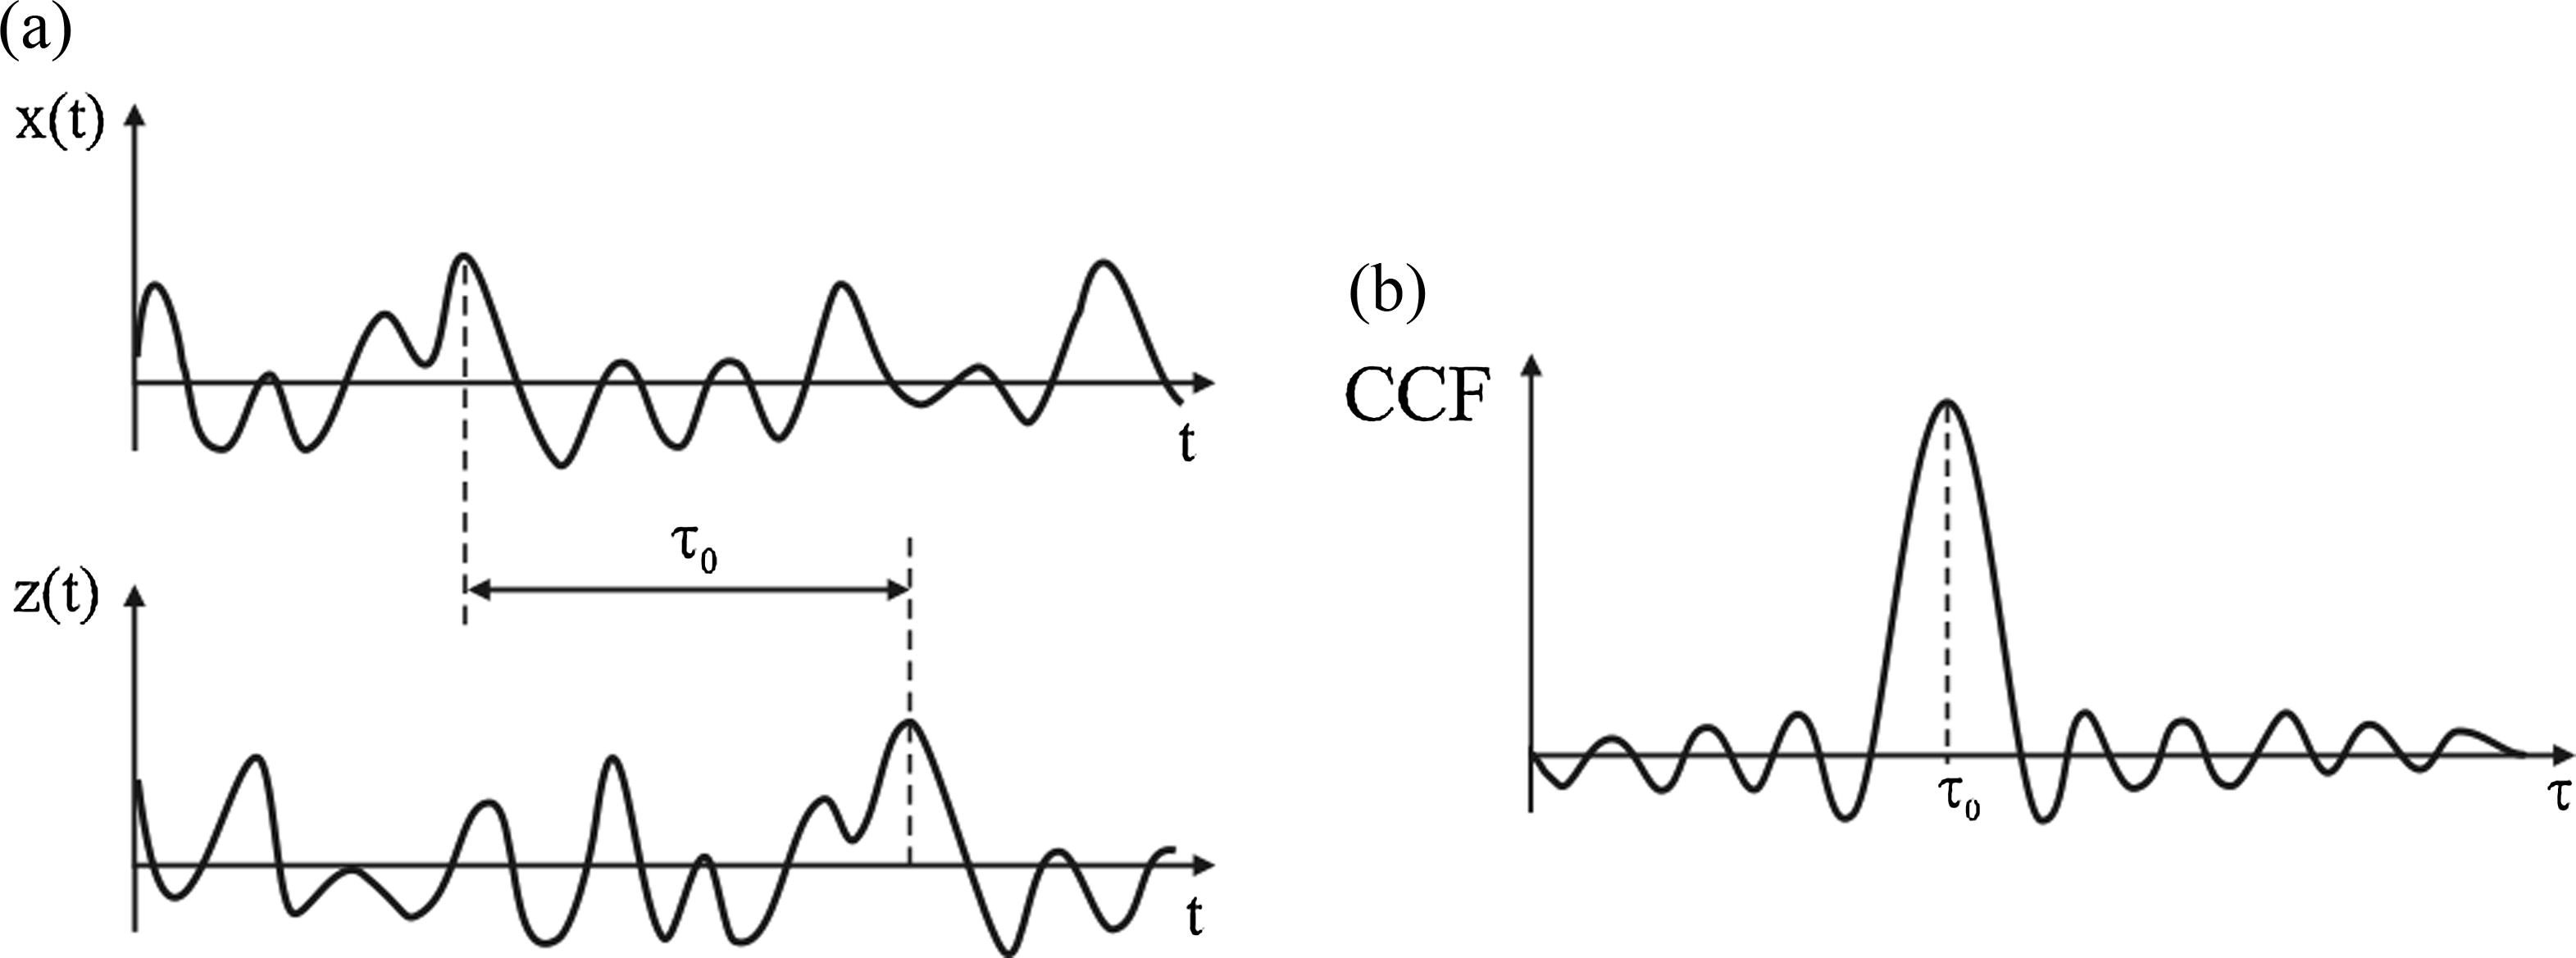
\includegraphics[width=1\linewidth]{figures/hanus diagram.jpg}
    \caption{Two figures illustrating CCF time delay determination. (a): Two arbitrary time series \(x(t)\) and \(z(t)\), which are well-approximated as identical time series with a time delay \(\tau_0\) between them. (b): A plot of the CCF applied to \(x(t)\) and \(z(t)\), showing maximum correlation at the time delay \(\tau_0\), representing the latency.}
    \caption*{Image Source: Hanus et al\cite{hanus2019}}
    \label{fig: Hanus CCF}
\end{figure}

\blindtext

